\documentclass[a4paper,twocolumn,11pt,unpublished]{quantumarticle}
\pdfoutput=1

\usepackage[utf8]{inputenc}
\usepackage[T1]{fontenc}
\usepackage[english]{babel}
\usepackage{amsmath,amssymb,amsfonts,mathtools,amsthm}
\usepackage{booktabs}
\usepackage{graphicx}
\usepackage{hyperref}

\newcommand{\ii}{\mathrm{i}}
\newcommand{\Id}{\mathbb{I}}
\newcommand{\ket}[1]{|#1\rangle}
\newcommand{\bra}[1]{\langle #1|}
\newcommand{\Sph}{\mathbb{S}}
\newcommand{\pauli}{\boldsymbol{\sigma}}
\newcommand{\bloch}{\boldsymbol{r}}
\newcommand{\axis}{\boldsymbol{v}}
\newcommand{\vstar}{\boldsymbol{v}_{\star}}
\newcommand{\norm}[1]{\left\lVert #1\right\rVert}
\newcommand{\argmaxop}{\operatorname*{arg\,max}}

\newtheorem{proposition}{Proposition}
\newtheorem{corollary}{Corollary}
\newtheorem{definition}{Definition}

\begin{document}

\title{Geometry-Aware Coherent Registerization of Single-Qubit Data Re-Uploading Models}

\author{L\'ea Cass\'e}
\affiliation{School of Computing and Mathematical Sciences, University of Waikato, Hamilton, New Zealand}
\affiliation{\'Ecole Polytechnique, Institut Polytechnique de Paris, Palaiseau, France}
\email{lc480@students.waikato.ac.nz}

\author{Bernhard Pfahringer}
\affiliation{School of Computing and Mathematical Sciences, University of Waikato, Hamilton, New Zealand}
\email{bernhard.pfahringer@waikato.ac.nz}

\author{Albert Bifet}
\affiliation{School of Computing and Mathematical Sciences, University of Waikato, Hamilton, New Zealand}
\affiliation{T\'el\'ecom Paris, Institut Polytechnique de Paris, Palaiseau, France}
\email{albert.bifet@waikato.ac.nz}

\maketitle

\begin{abstract}
Single-qubit data re-uploading models are usually terminated by measuring a fixed observable. We study their use as coherent internal modules. The interface has two stages. First, a quaternion representation of $SU(2)$ motion is used to separate gauge-only motion from observable state motion, after which a gauge-aware geometric construction selects a signed Bloch coordinate. Second, the selected coordinate is mapped to a projector probability, estimated coherently, decoded into a signed fixed-point register, and used to control a downstream quantum evolution without intermediate measurement. We prove the quotient-distance identity, the optimality and identifiability conditions of the tangent-axis estimator, and the registerization and downstream error bounds. Numerical controls validate the gauge correction and projection blindness. A complete Qiskit demonstrator implements coherent amplitude estimation, reversible phase-to-sign decoding, register-controlled evolution, and uncomputation. The construction establishes composability, but low-precision QAE remains strongly input dependent and the finite truth-table decoder is not scalable.
\end{abstract}

\section{Introduction}

A single-qubit Quantum Re-uploading Unit (QRU) prepares
\begin{equation}
\ket{\psi_\theta(x)}=U_\theta(x)\ket{0},
\qquad U_\theta(x)\in SU(2).
\end{equation}
Data re-uploading circuits are expressive one-qubit learners whose accessible frequency structure depends on their encoding generators and architecture~\cite{PerezSalinas2020,Schuld2021,Barthe2024}. They are nevertheless usually treated as terminal models: a fixed observable, commonly $Z$, is measured and converted into a classical scalar.

A composed quantum pipeline requires a different interface: the QRU output must be selected as a physically meaningful signed coordinate and transported coherently to a downstream routine. Figure~\ref{fig:qru_interface} summarizes the resulting architecture. The work does not introduce a new amplitude-estimation algorithm and makes no quantum-advantage claim.

\begin{figure*}[t]
\centering
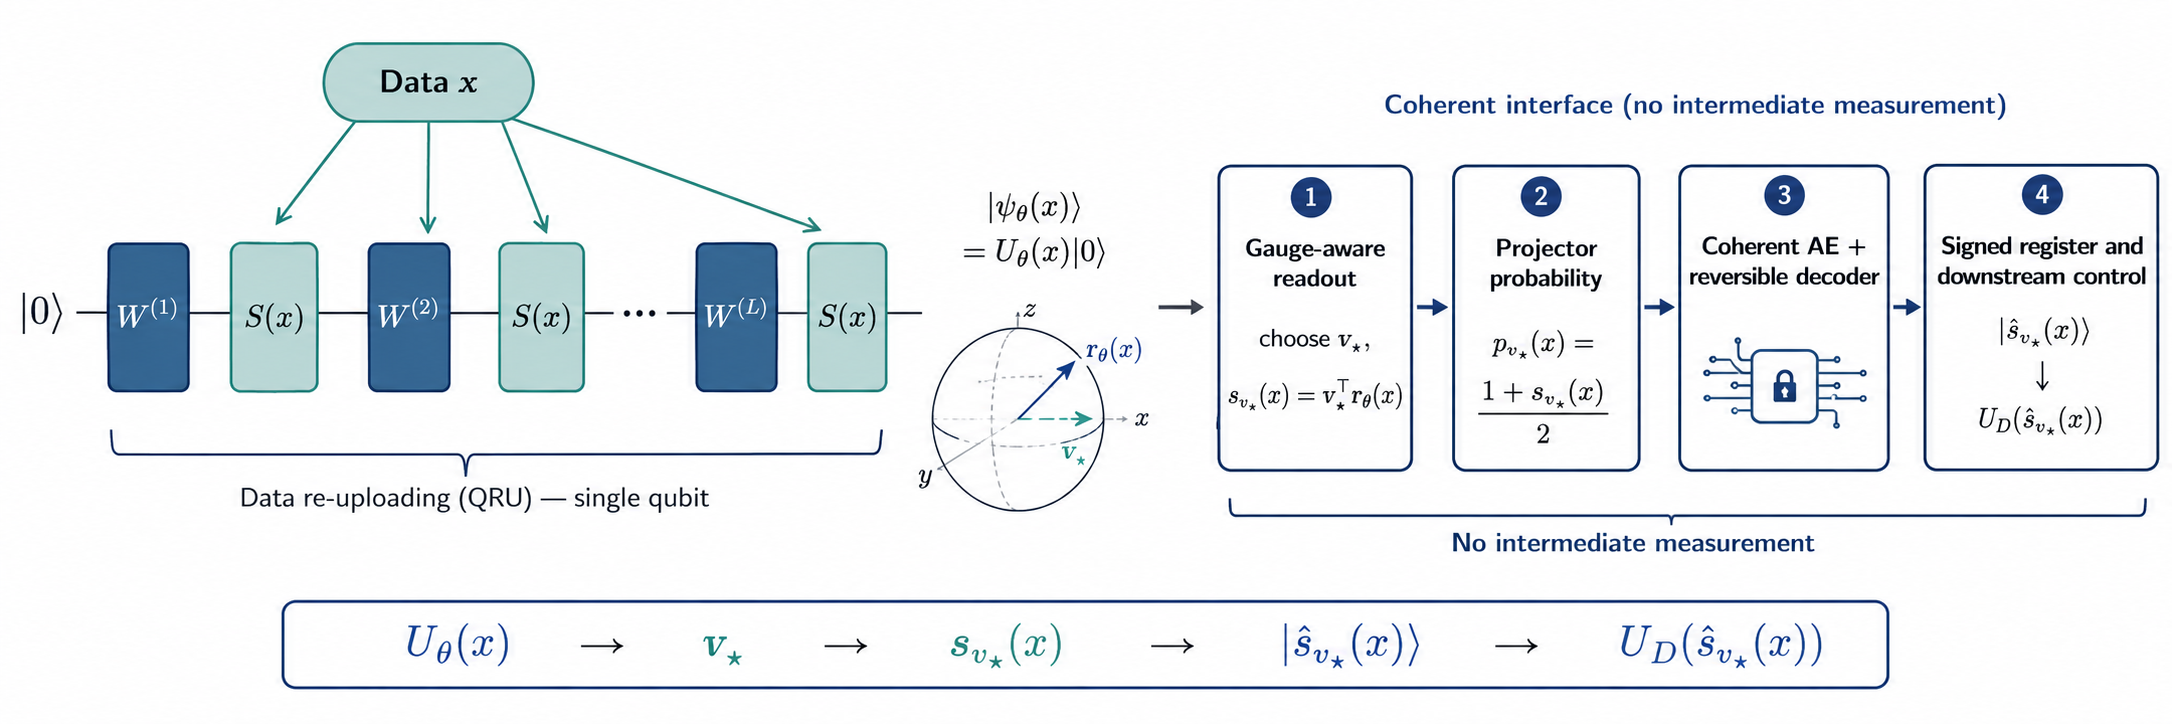
\includegraphics[width=\textwidth]{figures/qru_coherent_interface.png}
\caption{Overview of the proposed QRU interface. A single-qubit data re-uploading model prepares $\ket{\psi_\theta(x)}=U_\theta(x)\ket{0}$. A gauge-aware geometric readout selects the signed Bloch coordinate to expose, which is then converted into a projector probability, estimated coherently, decoded into a signed register and used as a downstream quantum control without intermediate measurement.}
\label{fig:qru_interface}
\end{figure*}

The first contribution is a gauge-aware signed-readout construction based on the observable QRU trajectory. The second is a coherent finite-precision interface that maps the selected readout to a quantum register and uses that register as a downstream control.

\section{Background and related work}

The QRU state has Bloch vector
\begin{equation}
\bloch_\theta(x)=
\bigl(\langle X\rangle_x,\langle Y\rangle_x,\langle Z\rangle_x\bigr)^T\in\Sph^2.
\end{equation}
For a unit axis $\axis\in\Sph^2$, define the signed readout
\begin{equation}
s_{\axis}(x)=\axis^T\bloch_\theta(x)
=\bra{\psi_\theta(x)}\axis\cdot\pauli\ket{\psi_\theta(x)}\in[-1,1].
\end{equation}
The conventional readout is $s_{e_z}=\langle Z\rangle$.

Every $U\in SU(2)$ admits the quaternion representation
\begin{equation}
U=\begin{pmatrix}\alpha&\beta\\-\beta^*&\alpha^*\end{pmatrix},
\quad
\alpha=q_0-\ii q_3,
\quad
\beta=-q_2-\ii q_1,
\end{equation}
with $q\in\Sph^3$ and $q\sim-q$. The unitary acts on Bloch vectors through the associated rotation in $SO(3)$, but the prepared pure state belongs to
\begin{equation}
SU(2)/U(1)\simeq\mathbb{CP}^{1}\simeq\Sph^2.
\end{equation}
Consequently, motion of the full unitary need not be observable in $U\ket{0}$.

For a selected axis, the directional projector
\begin{equation}
\Pi_{\axis}^{+}=\frac{\Id+\axis\cdot\pauli}{2}
\end{equation}
obeys
\begin{equation}
p_{\axis}(x)=\bra{\psi_\theta(x)}\Pi_{\axis}^{+}\ket{\psi_\theta(x)}
=\frac{1+s_{\axis}(x)}{2}.
\end{equation}
Coherent amplitude estimation can encode information about $p_{\axis}$ in a phase register using controlled oracle calls~\cite{Brassard2002,Rall2021,RallFuller2023}. Standard phase-estimation-based QAE returns a word $y\in\{0,\ldots,2^{m_\phi}-1\}$ whose amplitude estimate is
\begin{equation}
\widehat p_y=\sin^2\!\left(\frac{\pi y}{2^{m_\phi}}\right).
\end{equation}
This phase word is not a linear binary representation of $p_{\axis}$ or $s_{\axis}$; coherent use by another algorithm requires a reversible decoder.

\section{Gauge-aware signed-readout selection}

\subsection{Quotient geometry}

The relative rotation angle of two unit quaternions is
\begin{equation}
\delta_{\mathrm{rot}}(q_i,q_j)
=2\arccos\bigl(|q_i^Tq_j|\bigr).
\end{equation}
It is invariant under $q\mapsto-q$ but not under the stabilizer of $\ket{0}$. Define the quotient distance
\begin{equation}
\delta_{\mathrm{quot}}(U_i,U_j)
=\min_{\phi}\delta_{\mathrm{rot}}\bigl(U_i,U_jR_z(\phi)\bigr).
\end{equation}

\begin{proposition}[Quotient-state identity]\label{prop:quotient}
For $\ket{\psi_k}=U_k\ket{0}$,
\begin{equation}
\delta_{\mathrm{quot}}(U_i,U_j)
=2\arccos|\langle\psi_i|\psi_j\rangle|
=\arccos(\bloch_i^T\bloch_j).
\end{equation}
\end{proposition}

The first equality removes exactly the right $U(1)$ action that changes only the global phase of $U\ket{0}$. The second identifies this quotient with the pure-qubit Bloch geodesic distance. A proof is given in Appendix~\ref{app:proofs}.

The control $U(x)=VR_z(x)$ exposes the necessity of the quotient. Its raw rotation accumulates $2\pi$, while its quotient and Bloch-geodesic distances vanish numerically; see Fig.~\ref{fig:geometry}(a).

\subsection{Tangent-axis estimator}

For an ordered grid $x_1<\cdots<x_N$, let
\begin{equation}
D_i=\frac{\bloch_{i+1}-\bloch_i}{\Delta x_i},
\qquad
w_i\geq0,
\end{equation}
and define
\begin{equation}
C_w=
\frac{\sum_iw_iD_iD_i^T\Delta x_i}
{\sum_iw_i\Delta x_i}.
\end{equation}
The state-motion construction uses $w_i=\delta_{\mathrm{quot}}(U_i,U_{i+1})^2$, which equals Bloch-geodesic weighting by Proposition~\ref{prop:quotient}. Raw quaternion weights are retained only as an ablation.

\begin{proposition}[Optimal axis]\label{prop:axis}
For $\norm{\axis}=1$, the energy
\begin{equation}
E_w(\axis)=\axis^TC_w\axis
\end{equation}
is maximized by a principal eigenvector of $C_w$.
\end{proposition}

If $\lambda_1\geq\lambda_2\geq\lambda_3$ are the eigenvalues, we report
\begin{equation}
\Gamma=\frac{\lambda_1-\lambda_2}{\lambda_1+\eta}.
\end{equation}
The axis is rejected when $\lambda_1$ or $\Gamma$ falls below a fixed tolerance. Proposition~\ref{prop:axis} follows directly from Rayleigh--Ritz; the rejection condition prevents an arbitrary eigenvector from being interpreted as a physical direction when the covariance is null or degenerate. Since a principal eigenvector is defined up to sign, the signed interface uses the canonical orientation $k=\argmaxop_j |v_j|$ and $\axis\leftarrow-\axis$ if $v_k<0$.

\subsection{Validation and scope of the geometric claim}

The second analytic control uses $U(x)=R_z(x)R_y(\theta)$ on a restricted arc. Its $Z$ coordinate is constant while its state moves in the $XY$ plane. The identifiable geometric estimators recover an $XY$ direction, whereas $Z$ has zero tangent energy; see Fig.~\ref{fig:geometry}(b).

\begin{figure}[t]
\centering
\begin{minipage}{0.48\columnwidth}

\includegraphics[width=\linewidth]{figures/gauge_only_motion.pdf}
\centering\small (a)
\end{minipage}\hfill
\begin{minipage}{0.48\columnwidth}

\includegraphics[width=\linewidth]{figures/projection_blindness.pdf}
\centering\small (b)
\end{minipage}
\caption{Geometric controls. (a) Gauge-only $SU(2)$ motion produces raw rotation length while all Bloch coordinates remain constant. (b) A constant $Z$ readout hides observable motion in the $XY$ plane.}
\label{fig:geometry}
\end{figure}

For random QRUs, axes are fitted on $[-\pi,0]$ and evaluated on $[0,\pi]$ using one common state-motion energy. Quotient weighting is state-motion weighting by Proposition~\ref{prop:quotient}. Relative to unweighted Bloch PCA, its paired mean test-energy gain has a bootstrap interval excluding zero only at depth two; intervals include zero at depths three, five, and eight (Fig.~\ref{fig:results}(a)). The quotient construction is therefore a gauge-correct derivation of the state geometry, not evidence of a general quaternion-specific performance advantage.

To connect the geometric readout with the finite register interface, we use one reproducible depth-eight QRU diagnostic rather than a hand-picked visualization. The selected axis is accepted only when the tangent covariance is non-degenerate; for this instance,
\begin{equation}
\begin{aligned}
\vstar&=(-0.5939,\,0.6573,\,-0.4641)^T,\\
\Gamma&=0.3955.
\end{aligned}
\end{equation}
It is therefore not a disguised $Z$ readout. The projector identity is checked numerically through
\begin{equation}
\max_x\left|p_{\vstar}(x)-\frac{1+s_{\vstar}(x)}{2}\right|
=2.5\times10^{-16}.
\end{equation}

\begin{figure*}[t]
\centering
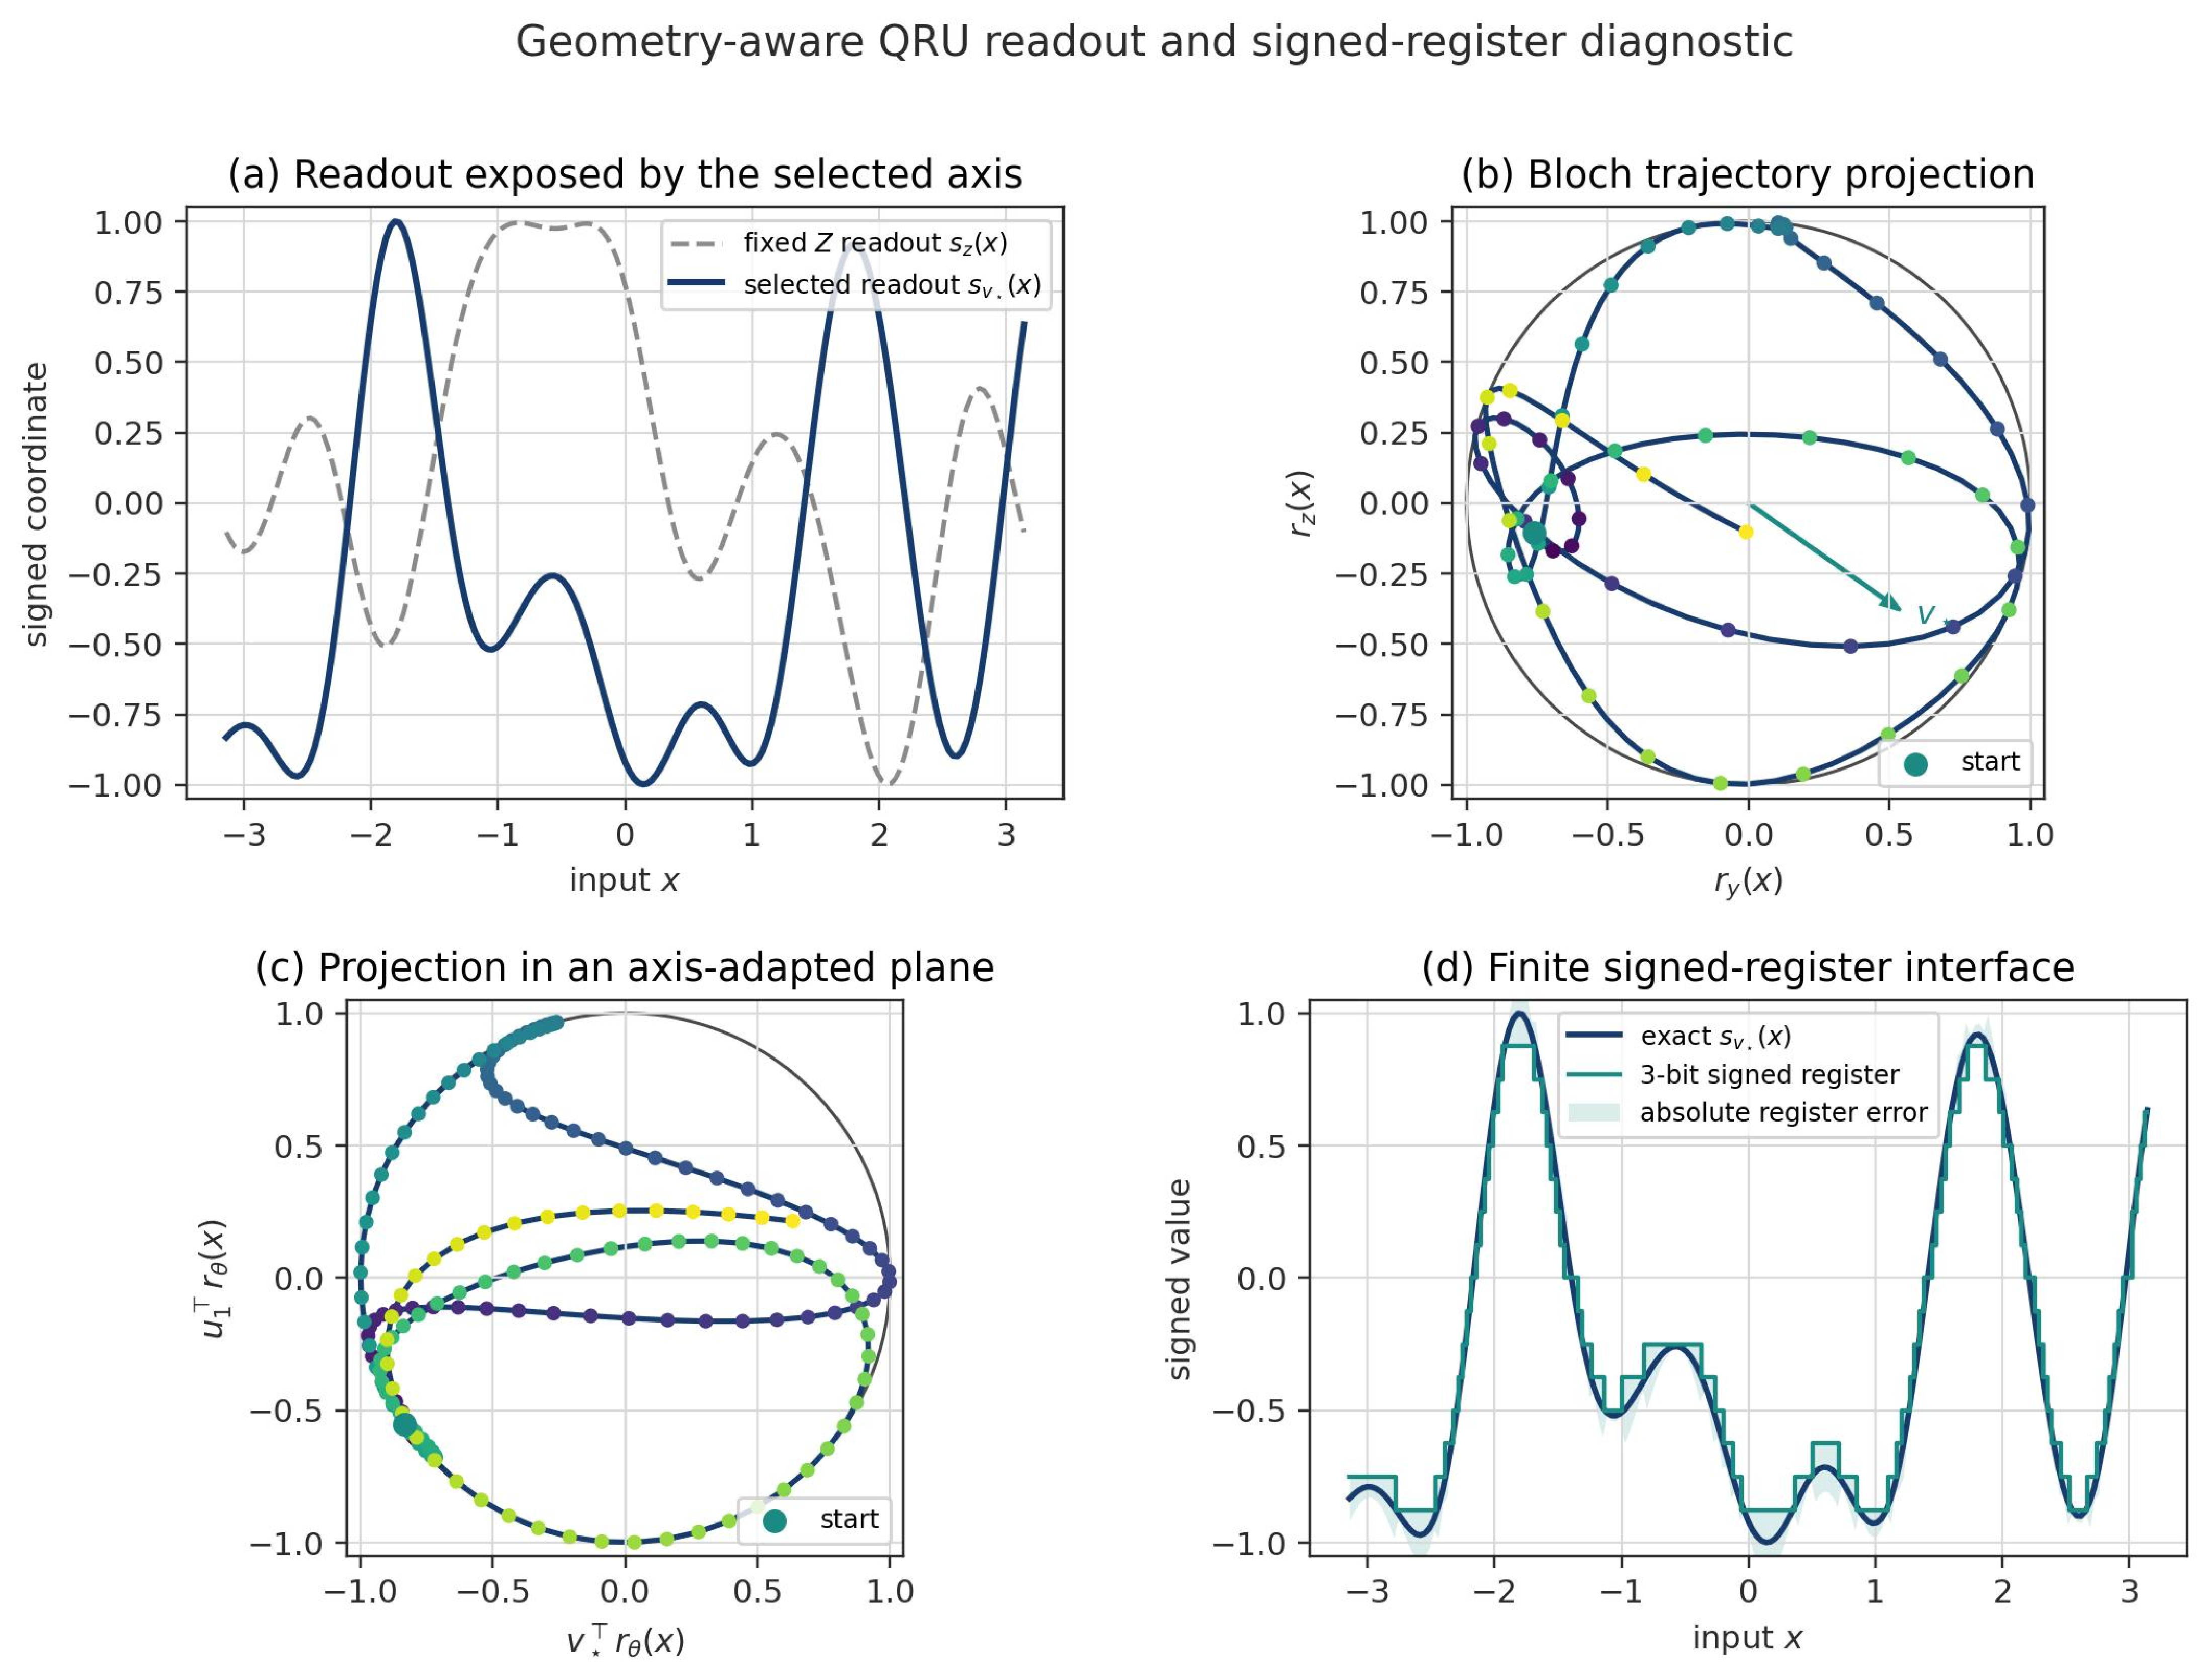
\includegraphics[width=0.92\textwidth]{figures/06_bloch_register_diagnostic.pdf}
\caption{\textbf{Bloch-register diagnostic.} Representative QRU instance linking the geometry-selected signed coordinate to its finite signed-register approximation. The selected axis gives a $2.35\times$ tangent-energy gain over $e_z$ and, for a three-bit signed register, a mean absolute signed error of $5.88\times10^{-2}$.}
\label{fig:bloch_register_diagnostic}
\end{figure*}

\section{Coherent signed-register interface}

\subsection{Signed registerization and error bounds}

We use canonical signed magnitude with one sign bit and $m_s$ fractional magnitude bits:
\begin{equation}
\widehat s=(-1)^b\sum_{k=1}^{m_s}b_k2^{-k},
\end{equation}
with sign bit zero for the numerical value zero and saturation at $1-2^{-m_s}$.

\begin{proposition}[Registerization error]\label{prop:error}
Assume $|\widetilde p-p|\leq\epsilon_p$, set $\widetilde s=2\widetilde p-1$, and quantize $\widetilde s$ to $\widehat s$. Then
\begin{equation}
|\widehat s-s|\leq2\epsilon_p+2^{-m_s}.
\end{equation}
For $U_D(s)=e^{-\ii\gamma sZ}$,
\begin{equation}
\norm{U_D(s)-U_D(\widehat s)}
=2\left|\sin\frac{\gamma(s-\widehat s)}{2}\right|
\leq|\gamma|\,|s-\widehat s|.
\end{equation}
\end{proposition}

The first inequality combines affine error propagation with fixed-point quantization; the second follows from the spectrum of $Z$ and $|\sin u|\leq|u|$.

\subsection{Coherent construction}

Choose $B_{\axis}$ such that
\begin{equation}
B_{\axis}^{\dagger}ZB_{\axis}=\axis\cdot\pauli.
\end{equation}
For $\axis=(\sin\theta\cos\phi,\sin\theta\sin\phi,\cos\theta)$, one valid choice is $B_{\axis}=R_y(-\theta)R_z(-\phi)$. A standard QPE-based QAE writes a coherent phase word $y$. A reversible finite decoder implements
\begin{equation}
\ket{y}\ket{0}
\longmapsto
\ket{y}\ket{\widehat s_y},
\qquad
\widehat s_y=Q_{m_s}\!\left[2\sin^2\!\left(\frac{\pi y}{2^{m_\phi}}\right)-1\right].
\end{equation}
The signed register controls
\begin{equation}
U_D^{\mathrm{reg}}
=\sum_z\ket{z}\!\bra{z}\otimes e^{-\ii\gamma s_zZ}.
\end{equation}
Because all $Z$ terms commute, each magnitude bit controls one weighted rotation and the sign bit reverses its direction. The signed register is then uncomputed. Circuit details are summarized in Appendix~\ref{app:circuit}.

\subsection{Functional validation, precision, and resources}

All signed words for $m_s=2,3$ reproduce the direct rotation with state infidelity below $4\times10^{-15}$. A seven-qubit two-input construction maintains a superposition of QRU branches, writes two signed values coherently, applies the downstream evolution, and reverses the pipeline. Its interference echo gives $P(0)>1-10^{-14}$; interface dephasing gives $P(0)=1/2$.

The complete QAE--decoder--downstream circuit is validated against a direct phase-word-controlled reference. For $(m_\phi,m_s)=(4,3)$, it uses ten qubits and attains fidelity above $1-1.4\times10^{-13}$ with signed-register reset probability above $1-1.3\times10^{-13}$. Naive decomposition gives depth 6156 and 2170 CX gates, dominated by the finite truth-table decoder.

The favourable point $p=0.3059$ is not representative. Over 201 uniformly spaced probabilities, mean signed errors for $(3,2),(4,3),(5,4)$ are $0.244$, $0.139$, and $0.0829$; only $1.5\%$, $4.5\%$, and $11.4\%$ of values achieve error at most $0.02$. Across 1488 random-QRU readouts, the corresponding means are $0.242$, $0.139$, and $0.0816$. The oscillatory phase-grid error and its downstream effect are shown in Fig.~\ref{fig:results}(b).

\begin{figure}[t]
\centering
\begin{minipage}{0.48\columnwidth}

\includegraphics[width=\linewidth]{figures/readout_generalization.pdf}
\centering\small (a)
\end{minipage}\hfill
\begin{minipage}{0.48\columnwidth}

\includegraphics[width=\linewidth]{figures/coherent_precision_robustness.pdf}
\centering\small (b)
\end{minipage}
\caption{Main numerical results. (a) Out-of-sample quotient/state weighting versus unweighted Bloch PCA. (b) Finite-precision QAE and signed-decoder error over the probability domain and QRU samples.}
\label{fig:results}
\end{figure}

\section{Discussion}

The two contributions solve distinct parts of one composability problem. Geometry determines which scalar coordinate is exposed; coherent registerization transports that coordinate without an intermediate classical interface. The geometric study also limits its own claim: quotient quaternion motion equals Bloch-geodesic state motion, and current random-QRU experiments do not establish systematic improvement over Bloch PCA. The remaining value of the quaternion formulation is the explicit diagnosis and removal of gauge-only motion.

The coherent circuit establishes functional composability, not near-term practicality. A measurement-reinjection pipeline may be preferable for one known classical input. Coherent transport becomes structurally relevant when inputs, scenarios, or downstream branches remain in superposition. Even then, standard low-precision QAE has strongly input-dependent errors, while the exact finite decoder scales exponentially in $m_\phi$. A scalable implementation requires structured reversible approximation of the sine-square map or an estimator producing a more directly consumable numerical representation. The present results therefore support an interface theorem and a verified small demonstrator, not a scalable NISQ architecture.

\section{Conclusion}

A QRU can be used as an internal quantum module only after defining both a meaningful signed output and a coherent transport mechanism. We introduced a gauge-correct tangent-axis construction, proved its quotient-state interpretation and spectral optimality, and showed that it detects projection blindness without supporting a general quaternion-specific advantage over Bloch PCA. We then implemented a coherent QRU-to-phase-to-signed-register-to-downstream pipeline with reversible decoding and uncomputation. The circuit is functionally correct and preserves interference, but its low-precision error and truth-table resource growth delimit the current claim. The next technical requirement is a structured reversible decoder and validation on trained QRUs.

\section*{Acknowledgment and Artifact Availability}
This work was conducted within the framework of the TAIAO project and University of Waikato. A reference implementation is available at: \url{https://github.com/LeaCasse/qru-quaternion-registerization}.

\appendix

\section{Proofs}\label{app:proofs}


\textit{Proof of Proposition~\ref{prop:quotient}.}
For unit quaternions $q_i,q_j\in\Sph^3$, let $q_{ij}=q_i^{-1}q_j$. Since $q_i^{-1}=\bar q_i$ and both quaternions are unit,
\begin{equation}
\operatorname{Re}(q_{ij})=q_i^Tq_j.
\end{equation}
Writing the relative rotation as $q_{ij}=\cos(\theta/2)+\boldsymbol n\sin(\theta/2)$ gives $\theta=2\arccos|q_i^Tq_j|$. The absolute value implements the projective identification $q\sim-q$. Hence $\delta_{\mathrm{rot}}$ measures the relative rotation in $SU(2)/\{\pm I\}\simeq SO(3)$; it is not invariant under the right stabilizer of $\ket{0}$.

Let $W=U_i^{\dagger}U_j$. Right multiplication by $R_z(\phi)$ changes the prepared state by
\begin{equation}
U_jR_z(\phi)\ket{0}=e^{-\ii\phi/2}U_j\ket{0},
\end{equation}
so minimizing over $\phi$ removes exactly the vertical $U(1)$ fibre of the ray $[U_j\ket{0}]$. The induced quotient distance between the two prepared rays is therefore
\begin{equation}
\delta_{\mathrm{quot}}(U_i,U_j)=2\arccos|\langle\psi_i|\psi_j\rangle|.
\end{equation}
For pure qubits,
\begin{equation}
|\langle\psi_i|\psi_j\rangle|^2=\frac{1+\bloch_i^T\bloch_j}{2}.
\end{equation}
The half-angle identity then gives
\begin{equation}
2\arccos|\langle\psi_i|\psi_j\rangle|=\arccos(\bloch_i^T\bloch_j),
\end{equation}
which is the Bloch geodesic distance. \hfill$\square$

\textit{Proof of Proposition~\ref{prop:axis}.}
In the continuous setting, the weighted readout-variation energy is
\begin{equation}
E_w(\axis)=\frac{\int w(x)\left|\frac{d}{dx}s_{\axis}(x)\right|^2dx}{\int w(x)dx},\qquad \norm{\axis}=1.
\end{equation}
Since $s_{\axis}(x)=\axis^T\bloch_\theta(x)$,
\begin{equation}
\frac{d}{dx}s_{\axis}(x)=\axis^T\bloch_\theta'(x),\qquad
E_w(\axis)=\axis^TC_w\axis,
\end{equation}
with
\begin{equation}
C_w=\frac{\int w(x)\bloch_\theta'(x)\bloch_\theta'(x)^Tdx}{\int w(x)dx}.
\end{equation}
The discrete estimator in Eq.~(14) is its finite-difference quadrature form. Since $C_w$ is symmetric positive semidefinite, the Rayleigh--Ritz theorem yields
\begin{equation}
\max_{\norm{\axis}=1}\axis^TC_w\axis=\lambda_1,
\end{equation}
attained by any principal eigenvector. If $\lambda_1=0$ the trajectory has no observable tangent energy; if $\lambda_1=\lambda_2$ the maximizing axis is not unique. The reported eigengap $\Gamma$ enforces identifiability before the axis is used as a signed interface. \hfill$\square$

\textit{Proof of Proposition~\ref{prop:error}.}
Since $s=2p-1$ and $\widetilde s=2\widetilde p-1$,
$|\widetilde s-s|=2|\widetilde p-p|\leq2\epsilon_p$. Signed-magnitude truncation with $m_s$ fractional bits has error at most $2^{-m_s}$, including endpoint saturation. The triangle inequality yields the first result. Diagonalizing $Z$ gives
$\norm{e^{-\ii\gamma sZ}-e^{-\ii\gamma\widehat sZ}}=\max_{z=\pm1}|e^{-\ii\gamma sz}-e^{-\ii\gamma\widehat sz}|=2|\sin(\gamma(s-\widehat s)/2)|$, which is bounded by $|\gamma||s-\widehat s|$. \hfill$\square$

\section{Coherent circuit construction}\label{app:circuit}

Let $A_{\axis}=XB_{\axis}U_\theta(x)$ so that $|\langle1|A_{\axis}|0\rangle|^2=p_{\axis}(x)$. The Grover operator is
\begin{equation}
Q_{\axis}=-A_{\axis}S_0A_{\axis}^{\dagger}S_{\mathrm{good}},
\end{equation}
where $S_0=\Id-2\ket{0}\!\bra{0}$ and $S_{\mathrm{good}}=\Id-2\ket{1}\!\bra{1}$. QPE applied to $Q_{\axis}$ yields the symmetric phases associated with $p_{\axis}=\sin^2\theta$. The finite decoder is a reversible lookup over the $2^{m_\phi}$ phase words. It is exact for the selected discretization but has exponential synthesis cost. After the controlled downstream operation, applying the decoder again returns all signed ancillas to $\ket{0}$.

\begin{thebibliography}{10}

\bibitem{PerezSalinas2020}
A.~P\'erez-Salinas, A.~Cervera-Lierta, E.~Gil-Fuster, and J.~I.~Latorre,
``Data re-uploading for a universal quantum classifier,''
\emph{Quantum} \textbf{4}, 226 (2020).

\bibitem{Schuld2021}
M.~Schuld, R.~Sweke, and J.~J.~Meyer,
``Effect of data encoding on the expressive power of variational quantum-machine-learning models,''
\emph{Phys. Rev. A} \textbf{103}, 032430 (2021).

\bibitem{Barthe2024}
A.~Barthe and A.~P\'erez-Salinas,
``Gradients and frequency profiles of quantum re-uploading models,''
\emph{Quantum} \textbf{8}, 1523 (2024).

\bibitem{Brassard2002}
G.~Brassard, P.~H\o yer, M.~Mosca, and A.~Tapp,
``Quantum amplitude amplification and estimation,'' in
\emph{Quantum Computation and Information}, AMS Contemporary Mathematics 305, 53--74 (2002).

\bibitem{Rall2021}
P.~Rall,
``Faster coherent quantum algorithms for phase, energy, and amplitude estimation,''
\emph{Quantum} \textbf{5}, 566 (2021).

\bibitem{RallFuller2023}
P.~Rall and B.~Fuller,
``Amplitude estimation from quantum signal processing,''
\emph{Quantum} \textbf{7}, 937 (2023).

\end{thebibliography}

\end{document}
